\documentclass[a4paper, 11pt]{article}
\setlength{\topmargin}{-0.5in}
\setlength{\textheight}{9.5in}
\setlength{\oddsidemargin}{-.1in}
\setlength{\textwidth}{6.5in}

\usepackage{multirow}
\usepackage{float}
\usepackage{array}
\usepackage[document]{ragged2e}
\usepackage{comment} 
\usepackage{subcaption}

\usepackage{datetime}

\newdateformat{mydate}{\monthname[\THEMONTH] \THEYEAR}

\newcolumntype{L}{>{\centering\arraybackslash}m{3cm}}

\usepackage{graphicx}
\graphicspath{{images/}}

\begin{document}


\LARGE\title{User Modeling in search for People with Autism}

\LARGE\author{Author: \textbf{Esha Massand}, Supervisor: \textbf{Keith Mannock}\\
\\
Birkbeck, University of London\\Department of Computer Science and Information Systems\\\\\\Project report submitted in partial fulfillment of the requirement for the \\MSc in Computer Science\date{\mydate\today}
\\\
}

\normalsize


\maketitle


\section*{Abstract}
\begin{justify}
This project report presents the development of a prototype web application to assist users with Autism when they search the web. The developed system models user interactions with the search process into a user profile by integrating insights from the core features of autism into the model. The user profile is applied to a synthesis of three leading search engines, and the entire system is integrated with an infra-red user interface component to assist users with Autism during search.\\
\end{justify}


\begin{justify}
This project is substantially the result of my own work, expressed in my own words, except where explicitly indicated in the text. I give my permission for it to be submitted to a Plagiarism Detection Service. This proposal may be freely copied and distributed provided the source is explicitly acknowledged.
\end{justify}

\begin{verbatim}














\end{verbatim}

\begin{center}
word count (project text only) :
\end{center}

\clearpage
\tableofcontents
\clearpage

\section*{Abbreviations}
\begin{tabular}{l l }
API & Application Programming Interface\\
AQ & Autism Quotient\\
ASD & Autism Spectrum Disorder\\
DSM & Diagnostic and Statistical Manual\\
GCS & Google Custom Search\\
HCI & Human Computer Interaction\\
HTTP & Hypertext Transfer Protocol\\
JSON & JavaScript Object Notation\\
IDE & Integrated Development Environment\\
KWIC & Key Word In Context\\
LEAP & LEAP Motion Controller\\
REST & Representational state transfer\\
RIFT & Oculus Rift Virtual Reality Head Mounted Display\\
TDD & Test Driven Development\\
UI & User Interface\\
UX & User Experience\\
VR & Virtual Reality\\
\end{tabular}

\section*{Definitions}

\begin{tabular}{l p{15cm}  }
Autism & Autism is amongst the most common neurodevelopmental condition and it is currently estimated that 1/68 children meet criteria for Autism Spectrum \cite{CDC}. Autism is five times more common amongst boys than girls (1/42 boys, and 1/189 girls). According to the Diagnostic and Statistical Manual (2013), Autism is characterized by persistent and early deficits in reciprocal social interaction and repetitive behaviours. Individuals vary from high functioning to low functioning (along a spectrum), with behaviours emerging around 2 to 3 years of age.
\end{tabular}
\clearpage

\section{Introduction}\label{intro}

This project report presents the development and evaluation of a prototype web-browser based application to assist users with Autism when they search the web, hereafter referred to as Jellibeans \footnote{Jellibeans are a rainbow of colours, different sizes and shades, and the name represents the difference in style of processing of individuals with ASD.}. Jellibeans will run in a web browser and utilises gesture and hand movement data recorded using the Leap Motion Controller (LEAP). 

Individual characteristics of each user will be measured using a 50 item questionnaire, the Autism Quotient (AQ \cite{Baron Cohen et al}) which measures tendency towards autistic traits. A score of 32 or higher indicates a strong likelihood of Autism or Asperger syndrome (the questionnaire has a 79\% sensitivity score). Individuals who score highly on the AQ will be offered the current user model for their search. The questionnaire data will be stored in the user's Google+ profile????

In programmatic terms, Jellibeans is designed to implement a research-based user model in search. This itself is a considerable part of the current research project and involves the development of a rule engine to transform the idiosyncratic ??? nature of search queries formed by individuals with ASD to work with current available search engines. This development involved collecting and analysing search behaviour patterns from people with and without ASD and building a set of transformation rules given the features of search queries that are formed by individuals with ASD.

Jellibeans will also improve the search experience for users with ASD by going one step further and enabling motion controlled search using the LEAP motion controller. The interface will be dynamic as opposed to static and this afford many advantages over traditional search engine interfaces.

\subsection {User Models in Search}

\subsection {Rule and Transformation Engine}

\subsection {Motion Controlled Navigation in Search}


\section {Aims}
The goal of the project is to build a prototype search tool that assists users with Autism search and navigate the web. To acheive this goal, the aims of this work are:

To synthesise the search results from three search engines, Google, Bing and Yahoo. For search results returned by Google, the Custom Search API will be used in line with the Google terms of service (as `screen scraping', or copying the data directly from the website is prohibited). It is a RESTful api with a single method called list. The API method used was GET, and the response data is returned as a JSON type. The response consists of (1) the actual search result, (2) metadata for search like number of  results, alternative search queries, and (3) custom search engine metadata. The data model depends on \cite{opensearch}.
For Bing and Yahoo search results, JSoup (a Java HTML parser) will be used to identify the links from the resulting query. The JSoup HTML parser was considered more effient for retrieving search results, as it reduced the number of lines of code required to complete the task. 
Jsoup has its advantages over html parsing. It contains a class representing a list of nodes, `Elements', which implements Iterable to iterate over a list in an enhanced for loop.
The resulting links are written to text file which stores the links in a text file in the projects source directory.

The system aims to deliver relevant results to the user, but what is ``relevant"? Not all users or groups of users search in the same way, so it is important to consider user intention. The first part of the current project aimed to investigate the differences between search queries of people with and without Autism, and to use those findings to build a stereotyped user model (a user model that will infer characteristics about the user from their diagnostic information) for a person with autism. Users will have to register will Google+ ???, and report their diagnostic information in the aboutMe section of their profile ??? / complete the Autism Quotient Questionnaire and obtain a score of autistic-like traits. Using the Google+ API, Jellibeans will connect to Google+ and ask the user to signin/ agree to the web application accessing their data. JavaScript will be used to parse the text in the aboutMe section to check if the user has identified as a persn with autism, aspergers, ASD or not. The result is returned via the console (inspect) command. ??? 

\section{Project Trailer}

\begin{figure}[H]
\begin{center}
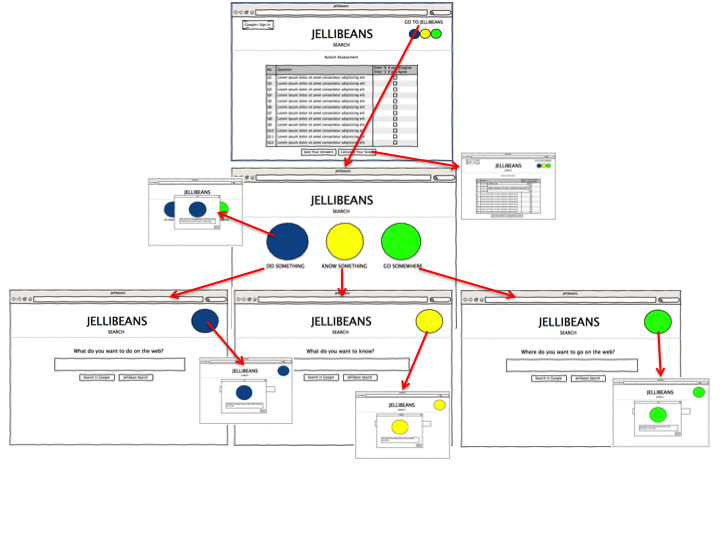
\includegraphics[scale=0.7]{JellibeanFlow.png}
\end{center}
\caption{Jellibean User Flow}
\label{JBeanUserFlow}
\end{figure}


\section {Background Research}\label{background} 
Search queries usually fall into one of three broad categories.  `Do' queries which characterise transactions between the user and the search engine, for example when the user wants to do something such as buy a plane ticket or listen to a song. There are also `Know' type queries. These are informational queries for example, the name of a band or restaurant in London. The third broad category is `Go' type queries, which are navigational in nature, for example, searching for a particular home page on the web. 

There are many stages to the search process. After identifying the information need, the user must formulate a search query. The user must browse through results once the query has been entered into a search engine. The whole process can be repeated if the user is not satisfied. The stage at which the user model will have most possible impact is before results are returned to the user, that is, at the query formulation stage. It is this stage that the user model will be implemeted (stage 2 on the user web-search process.)


\begin{center}
\begin{enumerate}
\item{Experience the need for an answer,
solution, or piece of information.}
\item{Formulate that need in a string of words and phrases, also known as “the query.”}
\item{Enter the query into a search engine.}
\item{Browse through the results for a match.}
\item{Click on a result}
\item{Scan for a solution, or a link to that solution.}
\item{If unsatisfied, return to the search results and browse for another link or ...}
\item{Perform a new search with refinements to the query}
\label{search flows}
\end {enumerate}

\hspace{1.5cm}
The User Web-Search Process \cite{seo}

\end{center}

\section{Core Feature 1: Research and Data Collection for a Combination Search Engine using Google, Yahoo and Bing.}

To implement the combination search engine I used three API’s provided by Google, Bing and Yahoo, namely, the Google Custom Search API, Yahoo BOSS Java API and Bing Search API. 

To get started with the Google Custom Search API, I created a project called ‘Jellibeans’ in the Google Developers Console, and an OAuth 2.0 Client ID. I obtained a Consumer Key and Secret to use the API, and used these in the application code to access the Google Custom Search Engine (see Figure~\ref{JBeanAppletGoogleCustomSearch1}). 

\begin{figure}[H]
\begin{center}
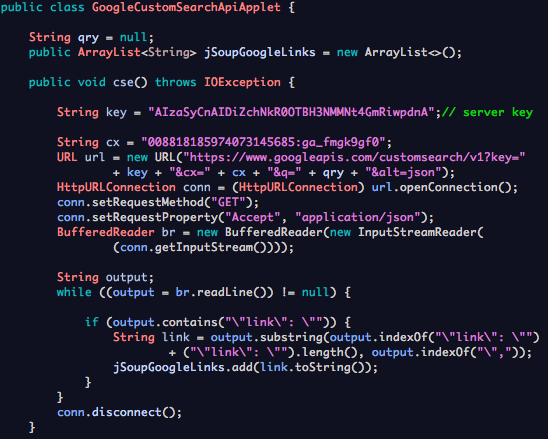
\includegraphics[scale=0.7]{JBeanAppletGoogleCustomSearch}
\end{center}

\caption{Jellibean Applet Combination Search Engine}
\label{JBeanAppletGoogleCustomSearch1}
\end{figure}

Following that I also registered my JavaScript origins within the console to access the Google+ API, and redirected URIs so that once users sign in using their Google+ login credentials they will be redirected to Jellibeans (or http://esha.mseth.co). This was done because I wanted users to be able to sign in and access their google profile from Jellibeans (see Figure~\ref{GoogleSignInPage}). 

\begin{figure}[H]
\begin{center}
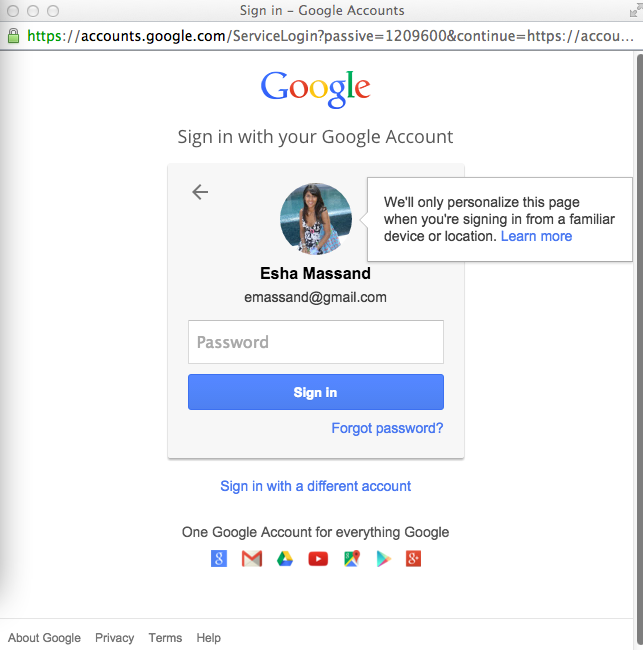
\includegraphics[scale=0.3]{GoogleSignIn}
\end{center}
\caption{Google Sign In Page.}
\label{GoogleSignInPage}

\end{figure}

Following a similar protocol for Yahoo and Bing Search API’s, I created projects in the Yahoo Developers Network, and Microsoft Azure Marketplace, and purchased an API Consumer Keys and Secrets (needed to use the APIs). 

\subsection{Web Scraping}
Web scraping was also an option, it quickly became a preferred because of integration of the three API’s and the flexibility/manipulation of  the resilts if they were returned using the same method. However this was against terms of service set out by Google (see section 5.3 of Figure~\ref{GoogleToS1}).

\begin{figure}[H]
\begin{center}
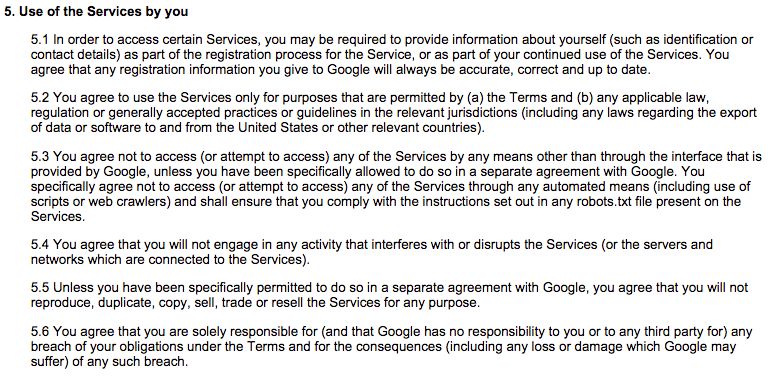
\includegraphics[scale=0.6]{GoogleToS}
\caption{Google Terms of Service}
\label{GoogleToS1}

\end{center}
\end{figure}


So, instead, I used the Jsoup API \cite{jsoup}, which is a java –written API for HTML. The library provides methods to conveniently extract data using DOM (Data Object Model) and CSS (Cascading Style Sheet) methods. The Jsoup HTML parser was used to scrape results only from Yahoo and Bing, and integrated these into a Java Applet that runs in Eclipse Luna IDE (see Figure~\ref{AppletFig}). The top 10 links, from each search engine were presented to users and ranked such that result 1 from Google was followed by result 1 from Yahoo, and that was followed by result 1 from Bing. Then results 2 from Google, Yahoo and Bing were presented and so on, until the 30 links were produced, in ranked order from the three search engines. 

\begin{figure}[H]
\centering
\begin{subfigure}{.5\textwidth}
  \centering
  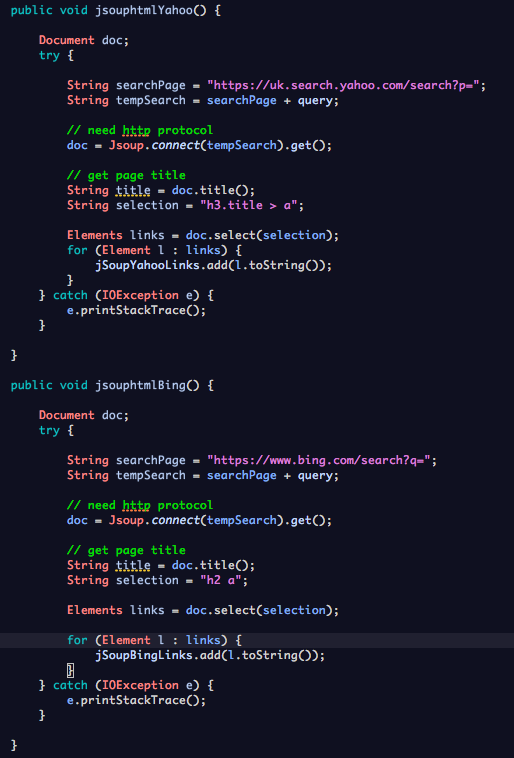
\includegraphics[width=.7\linewidth]{htmlParsers}
  \caption{JSoup HTML Parser.}
\end{subfigure}%
\begin{subfigure}{.5\textwidth}
  \centering
  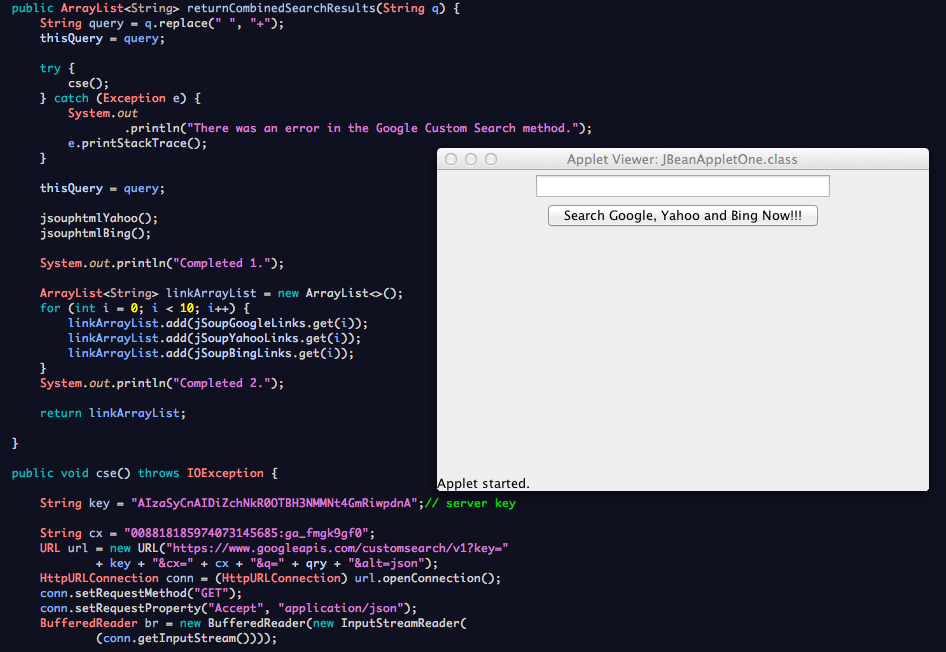
\includegraphics[width=.7\linewidth]{Applet}
  \caption{Complete query results.}
\end{subfigure}
\caption{JSoup HTML Parsers for Yahoo and Bing working with Google Custom Search API in Java Applet for testing.}
\label{AppletFig}
\end{figure}

\subsection{User Research and Testing of Core Feature 1}
To test the integrated combined search engine, the returned documents from 10 pre-determined search queries were presented to 10 participants who were identified as high AQ scorers. Participants were asked to comment on the search results that had been returned, and to choose three out of the links returned to follow up with, and to observe if anything was odd about the results returned. The responses from the 10 users were analysed to test core feature 1 and whether a combination search would be a good option for Jellibean Search, or whether it would introduce redundancy in the search results. 
Somewhat non-surprisingly (given the statistics of preferred search engines) the results revealed Bing Search was favoured the least, and Google results the most, with Yahoo falling somewhere in between. Out of the 30 responses participants indicated to follow up with, 21 were Google results, 3 were Yahoo, and 1 was Bing and 5 results overlapped between Google and Yahoo.
4 participants commented that the Bing results were distracting rather than helpful.

Given these findings from the user group, it was decided to continue using the Google results, but to drop the results from Yahoo and Bing, in line with the aim of the project as a whole – to improve returned search results for users with Autism.



\section{Core Feature 2: Building a User Model of Autism.}
To identify the features of the user model to build, I ran a study to collect example search queries on a set of informational needs from 37 participants. The participants were asked to give examples of search queries they would use to identify the name of a song they had heard (given the lyrics), or the name of a breed of a dog they had seen (given a picture of the dog). There were in total 10 search queries; the study was distrbuted widely via Surveymonkey.com \cite{surveymonkey} and can be seen in Appendix ~\ref{AppendixA}. Participants were also asked to complete the Autism Spectrum Quotient 50-item questionnaire see Appendix ~\ref{AQ}. The participants responses are analysed and reported back to surveymonkey.

The range of scores for the AQ is 0 to 50 with high scores indicating increased liklihood of autism-like traits. A score under 21 is a low to average result (many women average around 15 and men around 17). A score of 22-25 indicates autistic tendencies slightly above the population average. A score above 26 gives a borderline indication of high functioning autism, or aspergers. A score above 30 suggests a likelihood of Asperger syndrome or autism (sensitivity of test measure = 79\% \cite{Baron Cohen et al}).For the purposes of this study, individuals with scores equal to, and above 30 were interpreted as having `autistic-like traits'.

Participants were divided into two groups; low AQ scorers (scores below 30), and high AQ scorers (scores equal to and above 30). There were 30 low AQ scorers and 7 high AQ scorers. 


\subsection{Differences in Search Queries Between Users With and Without Autistic-like traits.}
I conducted a qualitative analysis on the search query strings from both low and high AQ scorer groups.

In both groups, Google was the prefered search engine by far, with all participants reporting that they used Google as a first choice. No one in the current sample used Yahoo or Bing. 
The low AQ scorer responses were analysed as a group. A baseline answer was generated using a frequency criterion of 40\% i.e., if 12 out of 30 respondents or more generated the same query string given an informational need, it was included in the model below. If two responses were equally as common, both are reported in the model. Data was discarded when a response indicated that the participant would do an image search, as this was not the aim of the survey. The results from the frequency analysis are presented below.

\begin{enumerate}
\item{You hear a song on the radio with the lyrics, ”Look at your children”, and you want to download it. What would you type into search on your favourite search engine to find out what song it was?\\\textit{Look at your children song}. \\\textit{Look at your children lyrics}.}
\item{You’ve lost touch with an old school friend (you went to St. Mary’s School). What key words/queries would you use to find them?\\\textit{St. Mary’s School Year of X}.}
\item{How would you identify what this is using a search engine (pretend you don’t know what it is called). What key words/queries would you use?\\\textit{Star shaped brown plant}.}
\item{How would you find out the name of this famous person using a search engine? What key words/queries would you use?\\\textit{Brown hair famous young women}.}
\item{How would you identify what breed this animal is using a search engine? What key words/queries would you use?\\\textit{Small dog fluffy breed}.}
\item{Your friend and you can’t agree on how Thandie Newton pronounces her first name. How would you resolve this using a search engine?\\\textit{Thandie Newton pronunciation}.}
\item{What would you search for to identify this pattern’s name, and which country it originates from?\\\textit{Repeating square maze pattern border}.}
\item{How would you search for delay’s relating to your (imminent) flight to Paris?\\\textit{Flight number, carrier, Paris, airport, flight time}.}
\end{enumerate}

The following observations were made for the users in the high AQ group:
\begin{enumerate}
\item{There were an increased number of imcompletely-formed queries. In the high AQ group, participants were more likely to miss off words in the query string. This was observed even though the sample size was much smaller in the high AQ group (7 people) compared to the low AQ group (29 people)). For example, when analysing the resuls from query 1 above, 2 out of 7 respondents in the high AQ group did not put `lyrics' or `song' in the search query when searching for the lyrics ``Look at your children". When these search strings are entered into Google, the results are very different (see Figure~\ref{someresults}). More results are returned to the incomplete query (302,000,000 compared to 32,900,000). The high AQ user group are presented with results that have a lower precision, i.e., more irrelevant information that they must sift through to find the answer to their search query.\label{incomplete}


\item{Although many high AQ scorers' formed query strings well, there was increased use of idiosyncratic words in the query strings that were forumulated. This is in line with previous research that suggests that people with autism organise information in more subjective and individual ways \cite{subjective organisation}. For example, referring to the picture of the dog as `yorkie pooh'(not listed in frequency index), `aeroplane' (frequency of 8254 words per million) instead of plane (frequency of 33900 words per million) or flight (29535 words per million) , `miniature' (less than 4973 words per million) instead of small (185463 words per million). The idiosyncratic nature of the words is captured by their lower frequency of use in the English language. Search engines use term frequency to determine if a document is relevant to the users search query. If the frequency of words used to form search queries differs between low and high AQ scorers, so will the rankings of the returned search results.}
\label{idiosyncracy}

\begin{figure}[H]
\centering
\begin{subfigure}{.5\textwidth}
  \centering
  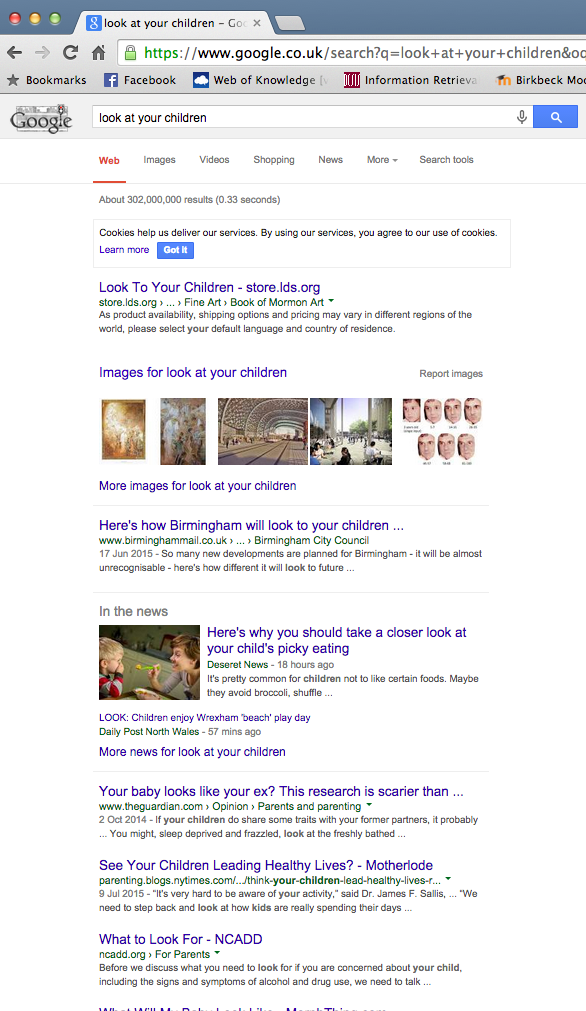
\includegraphics[width=.7\linewidth]{lookAtUrChildren}
  \caption{Incomplete query results.}
\end{subfigure}%
\begin{subfigure}{.5\textwidth}
  \centering
  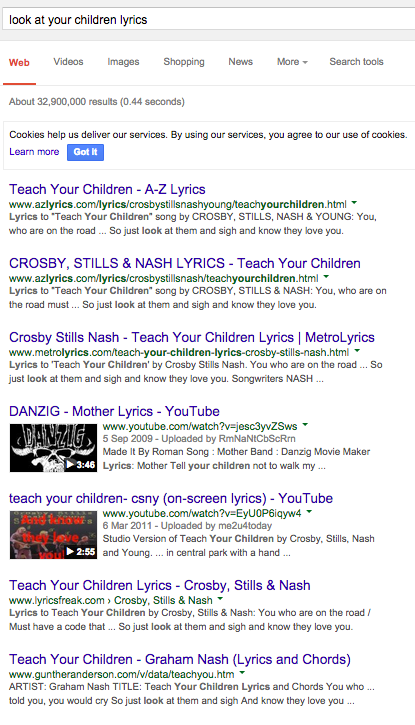
\includegraphics[width=.7\linewidth]{lookAtUrChildrenLyrics}
  \caption{Complete query results.}
\end{subfigure}
\caption{High and low AQ scorers both formed search queries accurately, however there was an increased tendency to omit the word ``lyrics" in the high AQ group resulting in very different search results.}
\label{someresults}
\end{figure}

\begin{comment}

\begin{figure}[H]
\begin{center}
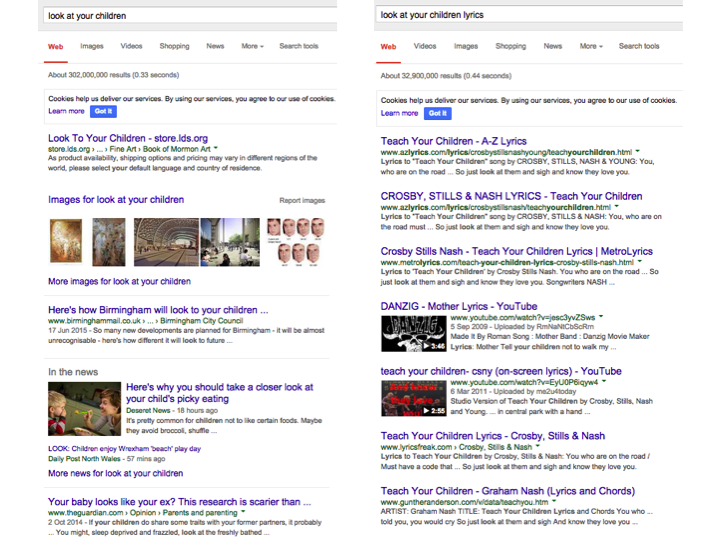
\includegraphics[scale=0.5]{LookAtYourChild}\\
\label{LookAtYourChild}
\end{center}
\end{figure}

\end{comment}
}

\item{One individual of the 7 individuals in the high AQ group demonstrated ambiguous use of third-person pronouns, which is characteristic of some individuals with Autism \cite{pronoun}. This includes using first names. This is particularly detrimental to search engine query strings because the use of names distrupts the term frequency - inverse document frequency weighting \cite{tfidf} of the search query and subsequently the results returned to the user.
}\label{pronoun}
 
\item{
For questions that were `social' in nature (e.g., featuring a face of a famous woman), 2 out of 7 individuals in the high AQ group indicated that these were types of queries that they would not normally be interested in, and so ``wouldn't bother asking it". This is, of course, in line with the characteristics of Autism according to \cite{DSM}. For these queries, it was more common for individuals in the high AQ group to include information in their search query string that was extraneous to the search question itself, compared to the low AQ group. For example, in query 4 above (which asked respondents to indicate how they would identify a famous person), 2 high AQ scorers included information about the woman's earing. Inevitably this `dilutes' the search query and results in reduced precision for the search engine.
}

\begin{comment}
\item{ 
Lastly there were more spelling errors and typographical errors in the high AQ group compared to the low AQ group.
}\label{spelling}
\end{comment}



\end{enumerate}


\section{Core Features 3 and 4: Jellibeans -- A Transformation Rule Engine}
Given the set of observations in the data reported above, the aims were to devise a set of rules that would `transform' queries made by individuals in the high AQ group to those similar to the low AQ group. The search engines already handle some of the observations from high AQ scorer queries. For example, the use of pronouns ('I' and `You') is already taken care of with the use of stop words, which is implemented by the search engine itself. The aim of the project is to therefore address issues that result in the search query string being misleading, and returning differnt results to low AQ scorer search queries. 

The aim for Jellibeans is to return search results that are more in line with low AQ scorers. In other words, search results from high AQ queries shared greater overlap with those made by the low AQ group, even though the queries were formed differently. The rule engine is thus a conrete and operationalised framework, for a theortetically-grounded user model of autism within search. \\

\vspace{5mm} %5mm vertical space
Jellibeans works to address more than one observation made during the data collection stage. As a general rule, changes will take the form of add on questions that aim to structure the individual to form a search query in a logical order so that key search terms are not dropped. The structure of the query's formation should also assist the user with less idiosyncratic search queries. \\

\vspace{5mm} %5mm vertical space
To address observation \ref{idiosyncracy} and to make high AQ scorer search queries less idiosyncratic, Jellibeans will prompt the user to categorise their search query into one of 4 possible types of queries, a `DO', `Know', `Go' or `Social' query. Each type of query will be associated with a colour, and this colour will be prominent on the page, to serve as a visual reminder of the task. This works to reduce the working memory load for the user, and to serve as a goal-directed que -- Two things we know are difficult for people with Autism are maintenance of information in working memory, and goal-directed tasks involving a high demand on Executive Functioning (Executive functions (also known as cognitive control and supervisory attentional system) is an umbrella term for the management (regulation, control) of cognitive processes, including working memory, reasoning, task flexibility, and problem solving as well as planning and execution \cite{EF}.) 

\vspace{5mm} %5mm vertical space
To address observation \ref{incomplete}, Jellibeans will have an intermittent `search' term box that confirms what the user wants to return. So, if the user wants to know something like lyrics of a song, or the name of a famous person, the price of an item for sale, they would enter `lyrics', `name' or `price' and this would be added to their search query (if it has not already been added by the user). This would ensure user search queries are more complete.

\vspace{5mm} %5mm vertical space
For observation \ref{pronoun}, pronouns (`I' and `You') are ignored via a stoplist which is implemented by the search engine itself. Jellibeans will also identify names of people via the third person library and suggest that these are removed, replaced with another search query term, or kept if the keyword is relevant. The extra layer of checking refines the search query.

\begin{comment}
\vspace{5mm} %5mm vertical space
Because Jellibeans bypasses the search engine interface, a spell checker will be implemented to address increased spelling errors in high AQ scorers (observation \ref{spelling}). This will also be in the form of a `suggestion' at the search query formulation stage.

\end{comment}

\vspace{5mm} %5mm vertical space

The Autism Quotient score of the user will be stored.

\section{Implementation}

\subsection{Use Case Diagram}

Feature uses

\begin{figure}[H]
\begin{center}
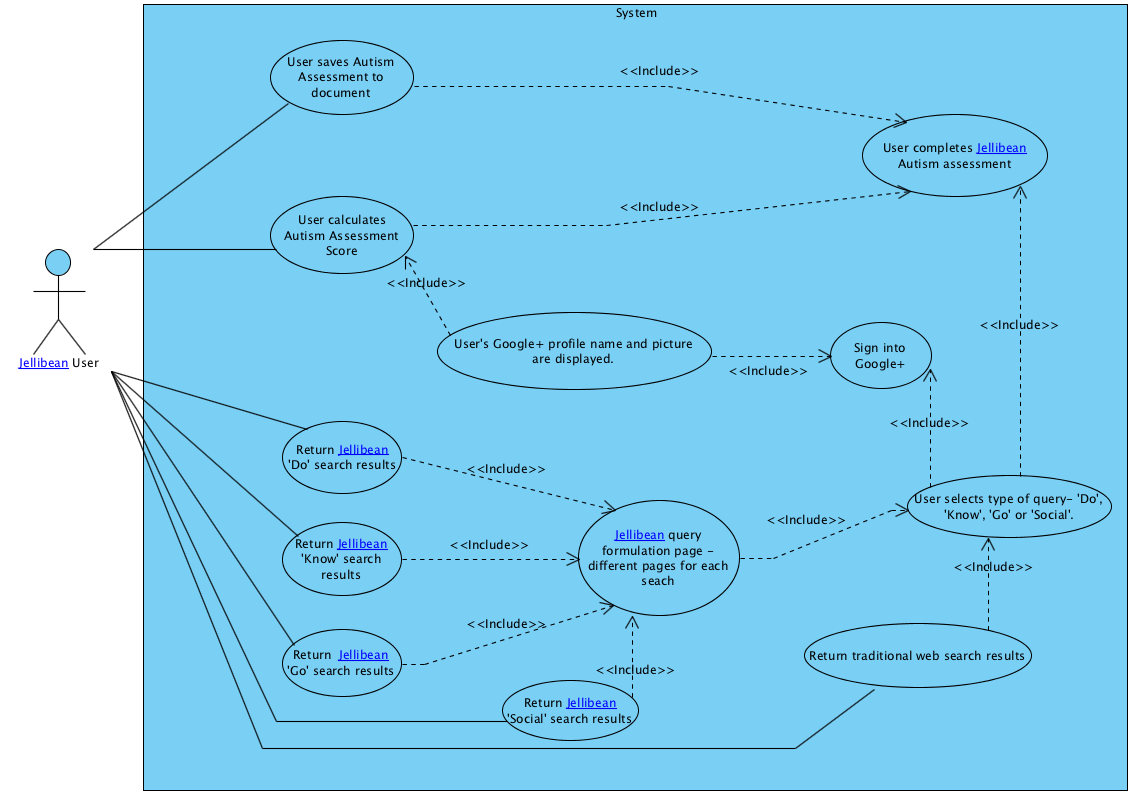
\includegraphics[scale=0.45]{JBeanUseCase}
\caption{Jellibean High Level UML Use Case Diagram}
\label{JBeanUseCase1}
\end{center}
\end{figure}

\subsection{Storage of information}
Google+ and storing to file on computer.
Returning AQ score to user.


\subsection{Classification of Users}
Classification used the AQ into high and low scorers and feeding that information back in a downloadable file/on the screen in an alert.

\subsection{Design Patterns (for web applications)}

Search engines like Google apply strong reduction techniques to navigation of the web. For example, one common way this reduction pattern is implemented is by assuming the behaviour of the current user is similar to the behaviour of other users in similar situations. This is often seen in recommendation engines, e.g., Amazon. The principle applied by Google is to ‘make it easy’ for the user \cite{googleTerms}, by assuming that users form search queries similarly, and returning similar results to those users.

As we have seen in the introduction, users with Autism behave in different ways to typical users when navigating search. Users with Autism do not use the same key phrases when looking for documents with several attributes, i.e., queries that would be best formulated using several iterations of search, or multiple search parameters. This leads to an ineffective search; one that requires users to sift through results which are in large-part irrelevant, and a bad user experience. Given the research findings observed in the current study, the parametric search pattern appears to be a better choice for the user group in question.  

Parametric search queries allow users to define parameters in an increasingly logical and structured way. As an example, consider the experience of searching for flights to a particular holiday destination, or for a person. This requires high cognitive ‘load’ (remembering and manipulating arrival, departure, destination, timings, airlines, seat preferences etc.) so searches are often structured using fixed options (see Figure~\ref{exped}).

\begin{figure}[H]
\begin{center}
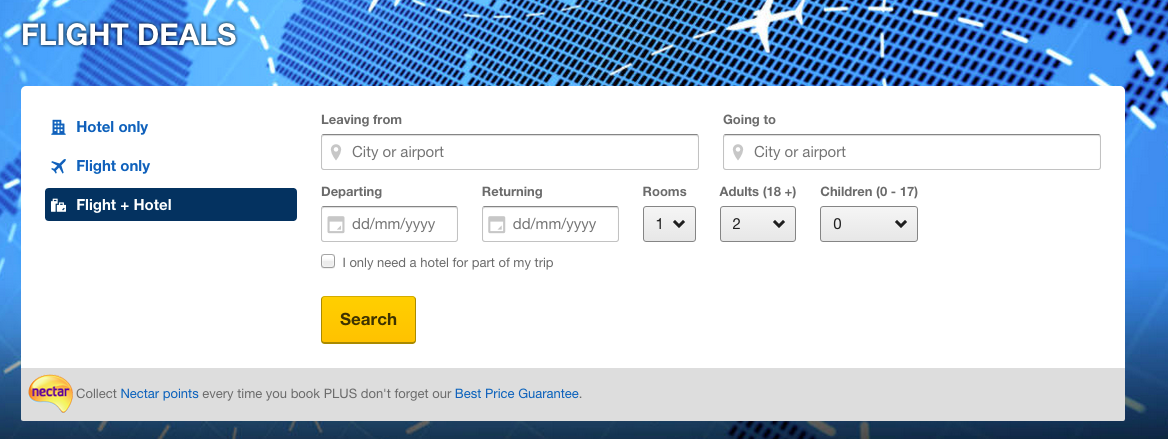
\includegraphics[scale=0.3]{expedia}\\

\caption{Expedia Parametric Search Example}
\label{exped}
\end{center}
\end{figure}

For typical users, parametric search is more structured, and in some circumstances seems more natural than a free – keyword search. It makes search queries easier to formulate in situations where there is a high cognitive load.  We can apply this idea to web search for people with Autism, by asking them to enter criteria that can be applied to subgroups of search queries. Parametric search can assist the user with capturing the search parameters that are useful for a query it does not ultimately reduce the number of search results returned; the possibility of a large result set is most definitely true. However, when used in addition to the original search query itself, the parametric search will refine the user’s search results in line with their search query, ultimately leading to a higher precision for the search enginei.

One of the aims of the study is to reduce the amount of textual information on the webpage presented to the user, so the solution implemented here tries to find a balance between these two aims.   


\subsection{What was actually done?}

\subsection{High Level UML Class Diagram of the System}

\begin{figure}[H]
\begin{center}
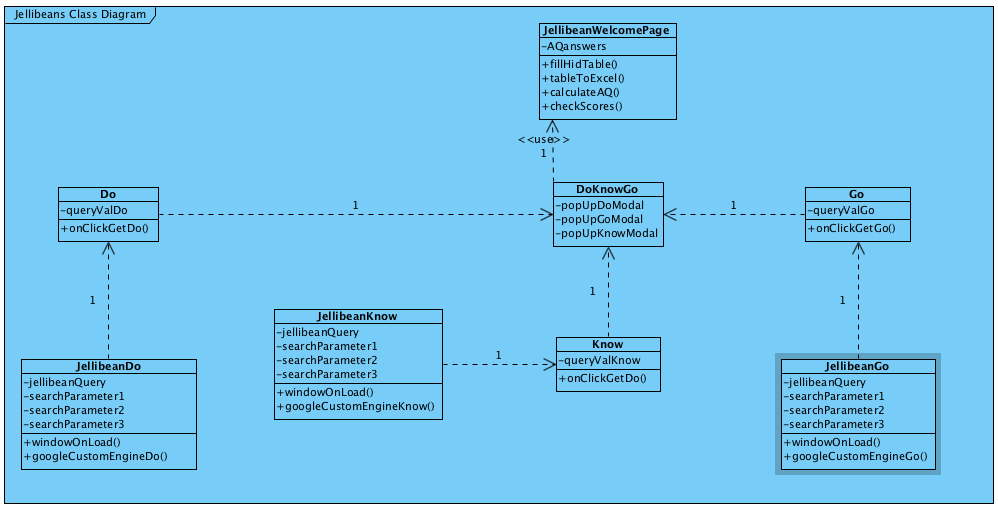
\includegraphics[scale=0.45]{jBeanClassDiagram}
\caption{Jellibean High Level UML Class Diagram}
\label{jBeanClassDiagram1}
\end{center}
\end{figure}

\subsection{API's and Development Tools}


\section{Core Feature 5: Integration with a Motion Controlled Interface.}
Integrating Jellibean with Motion Controller Hardware
LEAP motion controller and its use for the system.
Current Project’s Hardware Selection Process and Important Design Issues:
\begin{enumerate}
\item{Good timing correlates to a good meaning and User Experience.}
\item{The leap has options to ‘poll’ frames at a constant rate (to keep timing of movement accurate) which is important.}
\item{Cognitive ‘lag’ time. Each of our senses operates with a different lag time. Hearing has the fastest sense-to-cognition/understanding time, and surprisingly sight -- the slowest. If the devices interferes with the processing of the sense, it will confuse the combinatorial configuration of the senses, leading to misunderstandings in the meaning and a worse user experience.}
\item{Volume is important because this is a tool to be used with individuals with ASD, the device must have a low `volume’, i.e., the sensory experience cannot be overwhelming.}
\item{Load, by this I mean `cognitive' load is most desirable when not high. We do not want the device to be overwhelming in terms of it’s cognitive load.}
\item{Within the selection process, I did not just consider the physical design of the device, but also the way in which the devices manifests actions into behaviours. That is, how does the user engage behaviourally within the environment using the device? What about the physical sensation and its path towards a behavioural or emotional response? For example, can we program there to be an activity followed by a reward to reinforce the activity.}
\end{enumerate}

\subsection {Evaluation and Review of the Leap Motion Controller.}
Advantages
\begin{enumerate}
\item{Impressive}
\item{Uses infrared to embed the users (phantom) hand™ on the screen}
\item{New technology and novel to bring to laptops}
\item{East to set up}
\item{Has built in gestures and navigation tools}
\item{Can work in pretty dimly lit environments (but not all)}
\item{It is sophisticated (sometimes the polling frequency lets it down)}
\item{Picks up an impressive distance along the z axis}
\item{Offers a recalibration process if the controller is persistently jumpy, or there are discontinuities in the tracking data, if there are aberrations in the tracking data that occur in certain areas of the field of view, or poor tracking range. This can be done using the shiny surface such as the computer screen or mirror.}
\end{enumerate}	
Disadvantages
\begin{enumerate}
\item{Misses small hand movements}
\item{The range that it will detect is 150 degree angle along the y axis, this is reasonable but not always idea when gestures/hand movements are large.}
\item{Some parts of the screen the hands to not ‘reach’, i.e., bottom left /right of screen are sometimes hard to reach.}
\item{Loses the hand, stops working/sensing the hands, even when the controller stays on.}
\item{Often misses frames, so the user makes larger hand movements and then overshoots (when the LEAP catches up)}
\item{Built-in controls are not ideal}
\item{Lighting works best when the hand is seen in silhouette fashion by the controller. }
\end{enumerate}


\section{User Testing the System.}
The transformations that were implemented

\section{Conclusions and Discussion.}
Robots
Apache Lucene
Sandboxes
JavaScript html can't access third party pages
Yahoo and Bing was easier and faster to do html scraping


How does it compare to the original specification
This work has successfully completed aims XXX

\subsection{Signals of Quality Content}
I will test and evaluate the system. Testing will involve assessing the reliability and robustness of Jellibeans; the ease of its interaction; boundary conditions; ease of use; does it fullfil the aims of the project.
Evaluation of the system will include comparisons to existing search engines; assessing how this idea can be implemented to tailor an existing systems; assessing how well the system does compared to existing systems on a set of criteria that are only relevant to the user group in question (a collective measure of user happiness). Evaluation will also include quantitative metrics such as Recall, Precision, and False Negative/Positive rates.


Apache Solr\\

Future directions for the current project would be to develop an API or library for word frequencies in the written English language. These frequency data could have been used to suggest words that were more frequent in the written language for people with Autism, who tend to use idiosyncratic language. This would suggest alternatives for the user.\\

Alternatively, to use a thesaurus in the current project would be a useful addition.\\

Maybe google which has access to current trending searches would be able to have the `floating' modals to reflect the trends but the current version of Jellibeans is a working example of what could be achieved but with searches that are generally common, rather than trending.

colour blindness considerations - accessibility for people with Autism  



\clearpage
\begin{thebibliography}{100}
\bibitem{Baron Cohen et al} Baron-Cohen, Wheelrigjt, Skinner, Martin, Clubley (2001).   The Autism-Spectrum Quotient (AQ): evidence from Asperger Syndrome/high-functioning autism, males and females, scientists and mathematicians.  Journal of Autism and Developmental Disorders, 31, 5-17.
\bibitem{subjective organisation} Bowler, D. M., Gaigg, S. B., Gardiner, J. M. (2008). Subjective organisation in the free recall learning of adults with Asperger's syndrome. Journal of Autism and Developmental Disorders, 38(1), pp. 104-113. doi: 10.1007/s10803-007-0366-4 
\bibitem {DSM}Developmental Disabilities Monitoring Network Surveillance (2010) \textit{Centers for Disease Control and Prevention (CDC). Prevalence of autism spectrum disorders: Autism and Developmental Disabilities Monitoring Network, United States. MMWR Surveill Summ.2009; 58}, 10:1–20
\bibitem{EF} Executive Function, https://en.wikipedia.org/wiki/Executivefunctions, Retrieved 27 August 2015.
\bibitem{googleTerms} Google Privacy and Terms, http://www.google.com/policies/technologies/, Retrieved 27 August 2015.
\bibitem{jsoup} JSoup Java API, http://jsoup.org/, Retrieved 27 August 2015.
\bibitem{pronoun} Novogrodsky, R. (2013). Subject-pronoun use of Children with Autism Spectrum Disorders (ASD). Clinical Linguistics and Phonetics, 27(2), 85-93. 
\bibitem {opensearch}OpenSearch, http://www.opensearch.org/Specifications/OpenSearch/1.1, Retrieved 30 July 2015.
\bibitem{seo} Fishkin (2015) https://moz.com/beginners-guide-to-seo/how-people-interact-with-search-engines, Retrieved 3 August 2015.
\bibitem{surveymonkey}Surveymonkey, https://www.surveymonkey.com/home/, Retrieved 5 August 2015.
\bibitem{tfidf} Term Frequency Inverse Document Frequency Weighting, http://nlp.stanford.edu/IR-book/html/htmledition/tf-idf-weighting-1.html, Retrieved 9 August 2015.
\bibitem{wordfrequncy} Word Frequency Information, http://www.wordfrequency.info/free.asp?s=y, Retrieved 6 August 2015.
\end{thebibliography}





\newpage
\section {Appendices}

\newpage
\subsection{Search Query Survey} \label{AppendixA}

\begin{figure}[H]
\begin{center}
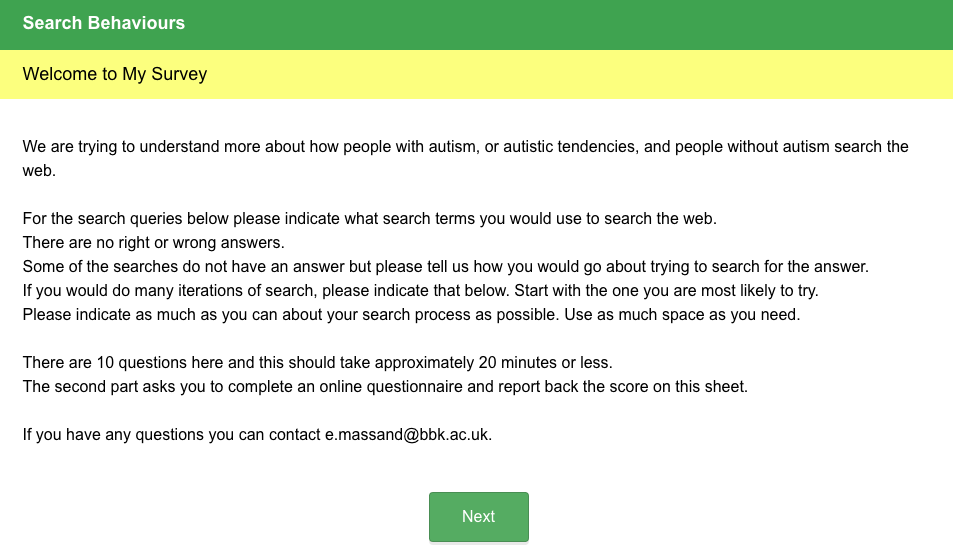
\includegraphics[scale=0.5]{survey1}\\
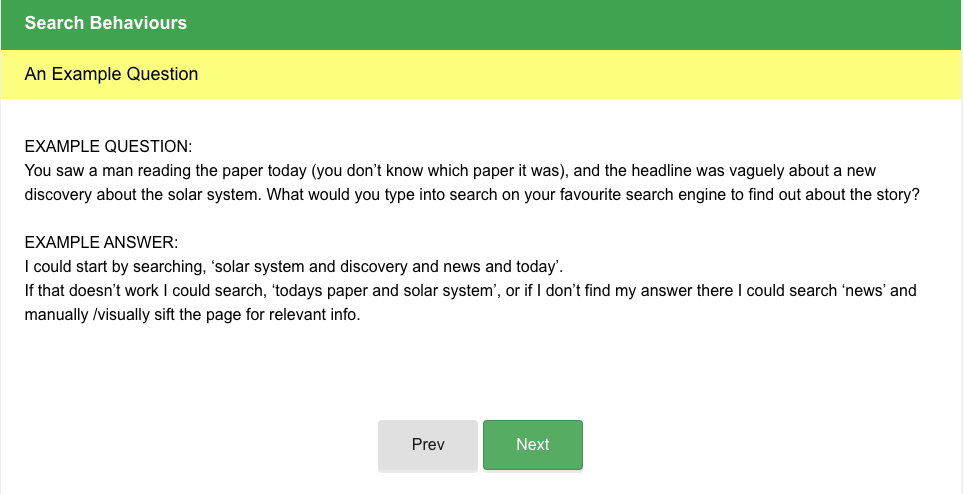
\includegraphics[scale=0.5]{survey2}\\
\end{center}
\end{figure}
\newpage
\begin{figure}[H]
\begin{center}
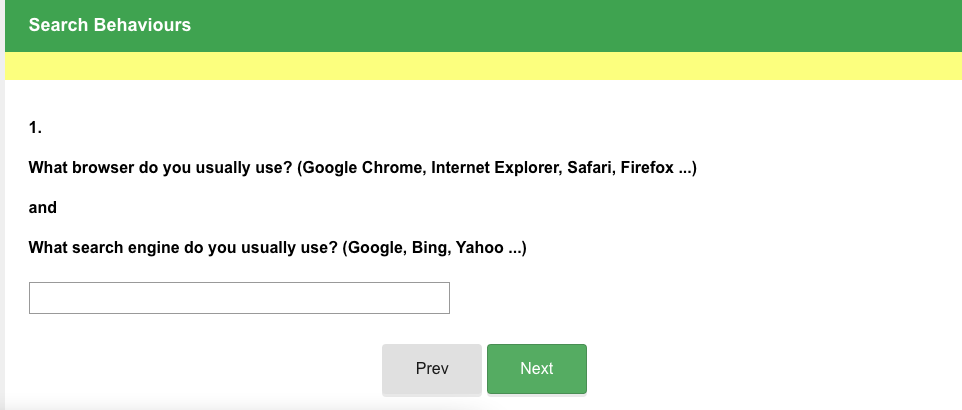
\includegraphics[scale=0.5]{survey3}\\
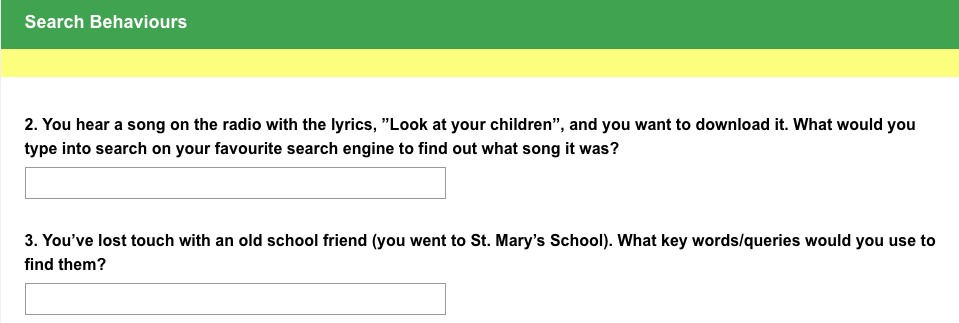
\includegraphics[scale=0.5]{survey4}\\
\end{center}
\end{figure}
\newpage
\begin{figure}[H]
\begin{center}
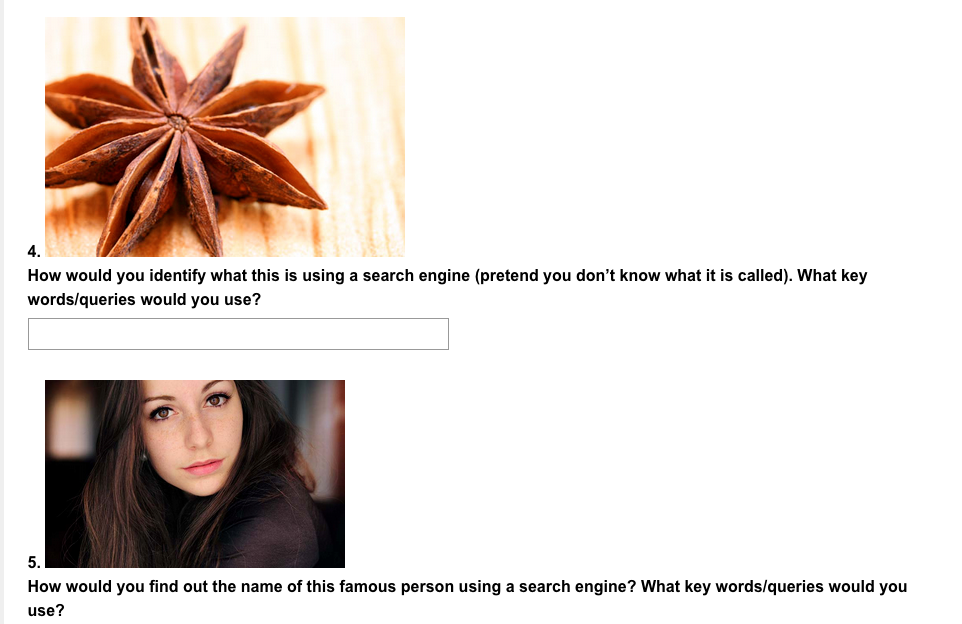
\includegraphics[scale=0.5]{survey5}\\
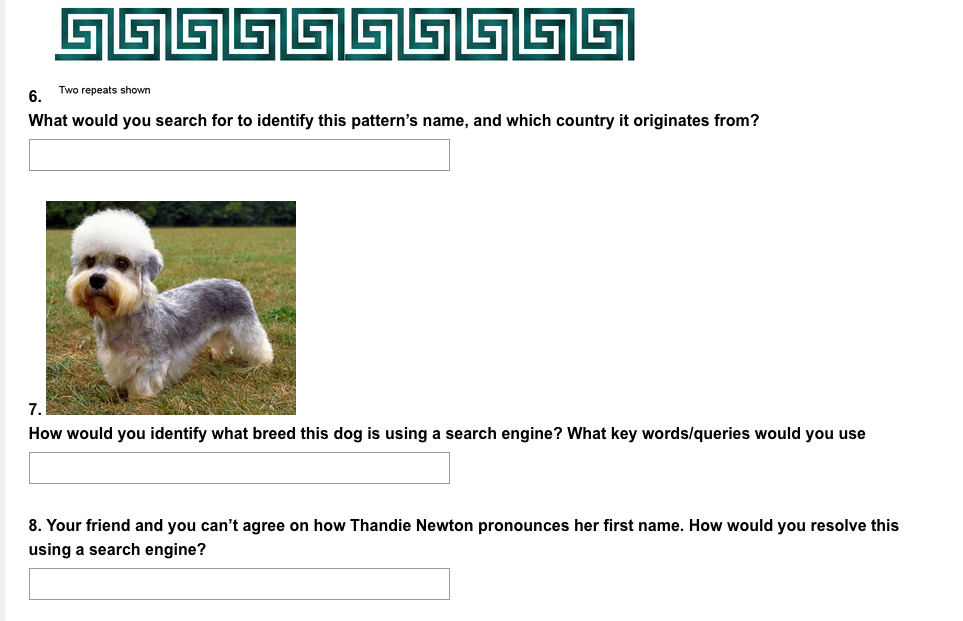
\includegraphics[scale=0.5]{survey6}\\
\end{center}
\end{figure}

\newpage
\begin{figure}[H]
\begin{center}
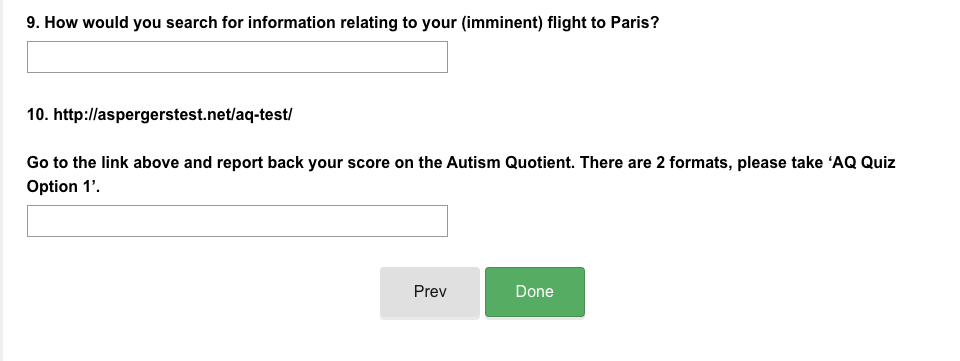
\includegraphics[scale=0.5]{survey7}\\
\caption{Search Query Survey on Surveymonkey.com \cite{surveymonkey}}
\end{center}
\end{figure}

\newpage
\subsection{Questions on the Autism Spectrum Quotient \cite{Baron Cohen et al}} \label{AQ}

Participants are asked to read each statement very carefully and rate how strongly they agree or disagree with the statement (Strongly Disagree, Slightly Disagree, Slightly Agree, or, Strongly Agree).  \\
\hspace{1cm}

I prefer to do things with others rather than on my own.\\
I prefer to do things the same way over and over again.\\
If I try to imagine something, I find it very easy to create a picture in my mind.\\
I frequently get so strongly absorbed in one thing that I lose sight of other things.\\
I often notice small sounds when others do not.\\
I usually notice car number plates or similar strings of information.\\
Other people frequently tell me that what I’ve said is impolite, even though I think it is polite.\\
When I’m reading a story, I can easily imagine what the characters might look like.\\
I am fascinated by dates.\\
In a social group, I can easily keep track of several different people’s conversations.\\
I find social situations easy.\\
I tend to notice details that others do not.\\
I would rather go to a library than a party.\\
I find making up stories easy.\\
I find myself drawn more strongly to people than to things.\\
I tend to have very strong interests which I get upset about if I can’t pursue.\\
I enjoy social chit-chat.\\
When I talk, it isn’t always easy for others to get a word in edgeways.\\
I am fascinated by numbers.\\
When I’m reading a story, I find it difficult to work out the characters’ intentions.\\
I don’t particularly enjoy reading fiction.\\
I find it hard to make new friends.\\
I notice patterns in things all the time.\\
I would rather go to the theatre than a museum.\\
It does not upset me if my daily routine is disturbed.\\
I frequently find that I don’t know how to keep a conversation going.\\
I find it easy to “read between the lines” when someone is talking to me.\\
I usually concentrate more on the whole picture, rather than the small details.\\
I am not very good at remembering phone numbers.\\
I don’t usually notice small changes in a situation, or a person’s appearance.\\
I know how to tell if someone listening to me is getting bored.\\
I find it easy to do more than one thing at once.\\
When I talk on the phone, I’m not sure when it’s my turn to speak.\\
I enjoy doing things spontaneously.\\
I am often the last to understand the point of a joke.\\
I find it easy to work out what someone is thinking or feeling just by looking at their face.\\
If there is an interruption, I can switch back to what I was doing very quickly. \\
I am good at social chit-chat.\\
People often tell me that I keep going on and on about the same thing.\\
When I was young, I used to enjoy playing games involving pretending with other children.\\
I like to collect information about categories of things (e.g. types of car, types of bird, types of train, types of plant, etc.).\\
I find it difficult to imagine what it would be like to be someone else.\\
I like to plan any activities I participate in carefully.\\
I enjoy social occasions.\\
I find it difficult to work out people’s intentions.\\
New situations make me anxious.\\
I enjoy meeting new people.\\
I am a good diplomat.\\
I am not very good at remembering people’s date of birth.\\
I find it very easy to play games with children that involve pretending.\\

\end{document} 